\documentclass[a4paper,14pt]{extarticle}

\usepackage[utf8x]{inputenc}
\usepackage[T1,T2A]{fontenc}
\usepackage[russian]{babel}
\usepackage{hyperref}
\usepackage{indentfirst}
\usepackage{here}
\usepackage{array}
\usepackage{graphicx}
\usepackage{caption}
\usepackage{subcaption}
\usepackage{chngcntr}
\usepackage{amsmath}
\usepackage{pgfplots}
\usepackage{pgfplotstable}
\usepackage[left=2cm,right=2cm,top=2cm,bottom=2cm,bindingoffset=0cm]{geometry}

\counterwithin{figure}{section}
\counterwithin{equation}{section}
\counterwithin{table}{section}
\newcommand{\sign}[1][5cm]{\makebox[#1]{\hrulefill}} % Поля подписи и даты
\graphicspath{{pics/}} % Путь до папки с картинками
\captionsetup{justification=centering,margin=1cm}
\def\arraystretch{1.3}

\begin{document}

\begin{titlepage}
\begin{center}
	\textbf{Санкт-Петербургский Политехнический Университет \\Петра Великого}\\[0.3cm]
	\small Институт компьютерных наук и технологий \\[0.3cm]
	\small Кафедра компьютерных систем и программных технологий\\[4cm]
	
	\textbf{ОТЧЕТ}\\ \textbf{о лабораторной работе}\\[0.5cm]
	\textbf{<<Исследование однокаскадных транзисторных усилителей>>}\\[0.1cm]
	\textbf{Электротехника и Электроника}\\[10.5cm]
\end{center}

\begin{flushright}
	\begin{minipage}{0.60\textwidth}
		\begin{flushleft}
			\small \textbf{Работу выполнили студенты}\\[3mm]
			\small группа 23501/4 \hspace*{17mm} Дьячков В.В.\\[3mm]
			\small группа 23501/4 \hspace*{17mm} Ламтев А.Ю.\\[5mm]
			
			\small \textbf{Преподаватель}\\[5mm]
		 	\small \sign[3.5cm] \hspace*{8mm} к.т.н., доц. Кочетков Ю.Д.\\[0.5cm]
		\end{flushleft}
	\end{minipage}
\end{flushright}

\vfill

\begin{center}
	\small Санкт-Петербург\\
	\small \the\year
\end{center}
\end{titlepage}

\section{Цель работы}

Овладеть методикой расчета и экспериментально исследовать основные параметры однокаскадных транзисторных усилителей, получить навыки настройки их режимов и снятия частотных характеристик усилителей.

\section{Чертеж схемы исследуемого устройства}

\begin{figure}[H]
\begin{center}
	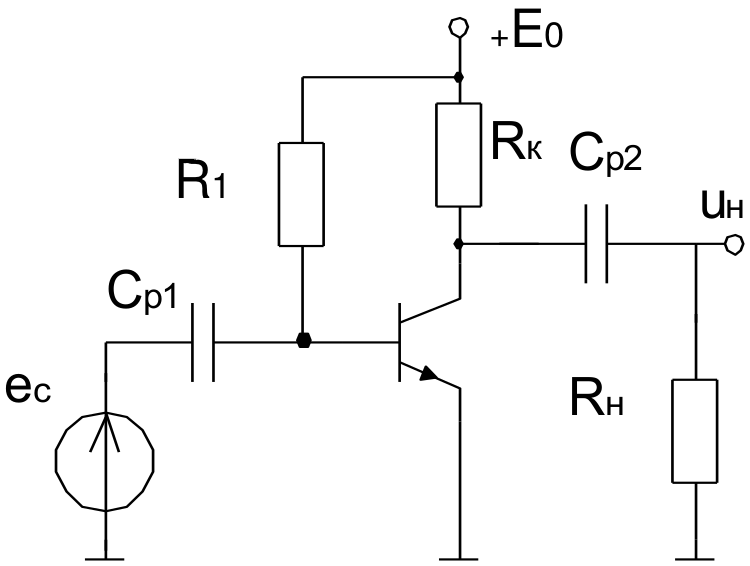
\includegraphics[width=7cm]{scheme}
	\caption{Схема однокаскадного усилителя}
\end{center}
\end{figure}

\section{Исходные данные}

Транзистор \verb+МП39+. Германиевый транзистор с $p-n-p$ переходом.

\begin{table}[H]
\begin{center}
	\caption{Исходные данные}
	\def\tabcolsep{10pt}
	\begin{tabular}{|c|c|c|c|c|c|c|c|c|c|}
		\hline
		$E_0$ &
		$U_\text{кэА}$ &
		$U_\text{бэ}$ &
		$R_\text{к}$ &
		$R_\text{н}$ &
		$C_{p1}$ &
		$C_{p2}$ &
		$f_{h21}$ &
		$C_\text{к}$ &
		$h_{21}$ \\
		\hline
		В &
		В &
		В &
		кОм &
		кОм &
		мкФ &
		мкФ &
		МГц &
		пФ &
		\\
		\hline
		8 &
		4 &
		0.2 &
		3.9 &
		2 &
		0.22 &
		0.47 &
		0.5 &
		60 &
		12 \\
	    \hline	
	\end{tabular}
	\label{tabular:1}
\end{center}
\end{table}

\newpage

\section{Теоретические расчёты}

Рассчитаем ток эмиттера транзистора: 
\[
I_\text{э} = \frac{(E_0 - U_\text{кэА})}{\frac{h_{21}}{1+h_{21}}R_\text{к}} = \frac{8 - 4}{\frac{12}{13} \cdot 3900} = 0.0011 \text{ А}
\]

Найдем сопротивление резистора $R_1$:
\[
R_1 = \frac{h_{21}(E_0-U_\text{БЭ})R_\text{к}}{E_0-U_\text{кэА}} = \frac{12 \cdot (8 - 0.2) \cdot 3900}{4} = 91260 \text{ Ом}
\]

Рассчитаем входное сопротивление:
\begin{equation}\label{eq:r_in}
R_\text{вх} \approx h_\text{11Э} = r_\text{б} + r_\text{э}(h_{21} + 1) = 50 + \frac{0.025}{0.0011} \cdot 13 = 345.45 \text{ Ом}
\end{equation}

Выходное сопротивление примем:
\begin{equation}
R_\text{вых} \approx R_\text{к} = 3.9 \text{ кОм}.
\end{equation}

Найдем коэффициент усиления по току:
\begin{multline}
K_{I0} = - h_{21} \cdot \frac{R_1}{R_1 + h_\text{11Э}} \cdot \frac{R_\text{к}}{R_\text{к} + R_\text{н}} =\\= - 12 \cdot \frac{91260}{91260 + 345.45} \cdot \frac{3900}{3900 + 2000} = - 7.90
\end{multline}

Рассчитаем коэффициент усиления по напряжению:
\begin{equation}\label{eq:k_u0}
K_{U0} = -\frac{h_{21} R_\text{к} R_\text{н}}{h_\text{11Э}(R_\text{к} + R_\text{н})} = -\frac{12 \cdot 3900 \cdot 2000}{345.45 \cdot (3900 + 2000)} = -45.92
\end{equation}

\newpage

\section{Экспериментально снятые зависимости}

\subsection{Амплитудная характеристика усилителя}

В таблице \ref{tab:ampl} и на рисунке \ref{tab:ampl} приведена амплитудная характеристика усилителя $U_\text{вых} = f(e_c)$. При значениях $e_c > e_{max} = 30.1$ можно заметить искажение входного сигнала. По полученным значениям было вычислено значение коэффициента усиления $K = 55.94$.

\begin{table}[H]
\begin{center}
	\caption{Зависимость напряжения $U_\text{вых}$ от $e_c$}
	\label{tab:ampl}
	\def\tabcolsep{40pt}
	\pgfplotstabletypeset[col sep=comma,
	    columns={e_c,u_out,k},
	    column type/.add={|c|}{},
	    columns/e_c/.style={fixed, column name={$e_c$, мВ}},
	    columns/u_out/.style={fixed, column name={$U_\text{вых}$, мВ}},
	    columns/k/.style={fixed, precision=2, zerofill, column name={$K$}},
	    every nth row={1}{before row=\hline},
	    every head row/.style={before row=\hline, after row=\hline},
	    every last row/.style={after row=\hline}
	   ]{data/ampl.csv}
\end{center}
\end{table}

\begin{figure}[H]
\begin{center}
	\begin{tikzpicture} [every plot/.append style={thick}]
		\begin{axis}[
			height=0.4\textheight,
			width=0.9\textwidth,
			legend pos=north west,
			xlabel={$e_c$, мВ},
			ylabel={$U_\text{вых}$, мВ},
			xlabel near ticks,
			ylabel near ticks,
			xmin = 0,
			xmax = 50,
			ymin = 0,
			ymax = 3000,
			grid=major
		]
		\addplot table[x=e_c,y=u_out,col sep=comma]{data/ampl.csv};
		\addplot table[x=e_c,y=u_out,col sep=comma]{data/ampl_theory.csv};
		\addplot +[mark=none, dashed, black, samples=2] coordinates {(30,0) (30,3000)};
		\legend{Эксп., Teор.}
		\end{axis}
	\end{tikzpicture}
	\caption{Зависимость напряжения $U_\text{вых}$ от $e_c$}
	\label{fig:ampl}
\end{center}
\end{figure}

\newpage

\subsection{Логарифмическая амплитудно-частотная характеристика усилителя}

В таблице \ref{tab:bode} и на рисунке \ref{fig:bode} приведена амплитудно-частотная характеристика усилителя при $e_c = \frac{e_{max}}{2} \approx 20$ мВ.

\begin{table}[H]
\begin{center}
	\caption{ЛАЧХ усилителя}
	\label{tab:bode}
	\def\tabcolsep{25pt}
	\pgfplotstabletypeset[col sep=comma,
	    columns={f,u_out,k,lg_k},
	    column type/.add={|c|}{},
	    columns/f/.style={fixed, column name={$f$, Гц}},
	    columns/u_out/.style={fixed, column name={$U_\text{вых}$, В}},
	    columns/k/.style={fixed, zerofill, column name={$K$}},
	    columns/lg_k/.style={fixed, precision=4, zerofill, column name={$20 \cdot \lg K$, дБ}},
	    every nth row={1}{before row=\hline},
	    every head row/.style={before row=\hline, after row=\hline},
	    every last row/.style={after row=\hline}
	   ]{data/bode.csv}
\end{center}
\end{table}

\begin{figure}[H]
\begin{center}
	\begin{tikzpicture} [every plot/.append style={thick}]
		\begin{axis}[
			height=0.4\textheight,
			width=0.9\textwidth,
			legend pos=north west,
			xlabel={$f$, Гц},
			ylabel={$20 \cdot \lg K$, дБ},
			xlabel near ticks,
			ylabel near ticks,
			xmode=log,
			log basis x=2,
			xtick={8, 32, 128, 512, 2048, 8192, 32768, 131072, 524288},
			xmin=8,
			xmax=524288,
			ymin=-15,
			ymax=35,
			grid=major
		]
		\addplot table[x=f,y=lg_k,col sep=comma]{data/bode.csv};
		\addplot table[x=f,y=lg_k,col sep=comma]{data/bode_theory.csv};
		\legend{Эксп., Teор.}
		\end{axis}
	\end{tikzpicture}
	\caption{ЛАЧХ усилителя}
	\label{fig:bode}
\end{center}
\end{figure}

\subsection{Измерение входного и выходного сопротивления}

Для измерения входного сопротивления усилителя последовательно с источником сигнала, был включен измерительный резистор $R_\text{изм} = 330$ Ом, при этом $e_c = 20$ мВ, а $U_\text{вx} = 9.41$ мВ:
\[
R_\text{вх} = \frac{U_\text{вх} \cdot R_\text{изм}}{e_c - U_\text{вх}} = \frac{9.41 \cdot 330}{20 - 9.41} = 293.2 \text{ Ом}
\]

Для измерения выходного сопротивления усилителя, от выхода схемы отключался $R_\text{н}$:
\[
R_\text{вых} = \frac{(U_\text{вых хх} - U_\text{вых Rн}) \cdot R_\text{н}}{U_\text{вых Rн}} = \frac{(1.2 - 0.44) \cdot 2000}{0.44} = 3454 \text{ Ом,}
\]
где $U_\text{вых хх}$ - сопротивление выходного сигнала при отсутствии резистора $R_\text{н}$, $U_\text{вых Rн}$ - сопротивление выходного сигнала при подключенном резисторе $R_\text{н}$.

\newpage

\section{Уточнение теоретических величин}

При установлении на схеме сопротивления резистора $R_1 = 91.26$ кОм, которое было посчитано с использованием заданного значения $h_{21} = 12$, значение $U_\text{кэА} = 4.12$ В, что имеет отклонение не выше $\pm 10 \%$ от заданного \linebreak $U_\text{кэА} = 4$ В. Поэтому $h_{21}$ не нуждается в уточнении.

Получив экспериментальное значение $R_\text{вх} = 293.2$ Ом и с учётом того, что $h_{11\text{Э}} \approx R_\text{вх}$, вычислим уточнённое значение $K_{U0}$: 

\[
K_{U0} = \frac{h_{21}R_\text{н}R_\text{к}}{h_\text{11Э}(R_\text{к}+R_\text{н})} = \frac{12 \cdot 3900 \cdot 2000}{293.2 \cdot 5900} = 54.1
\]

Таким образом, 
\[
K_{U0\text{ теор.}} = 54.1 \approx 55.94 = K_{U0\text{ эксп.}}
\]

\section{Выводы}

Вычесленные уточнённые теоретические и полученные экспериментальные значения близки. А значит, формулы \ref{eq:r_in} -- \ref{eq:k_u0} могут быть использованы.

\end{document}
